\section{Reactive Programming}
In diesem Kapitel geht es rund um das Verstehen von \textbf{Reactive Programming}. Da es im Netz nur wenig Material zum Einstieg gibt bzw. das Thema meist nur oberflächlich angekratzt wird und die offizielle Dokumentation nur den Wenigsten zum Einleuchten bringt, wird in dieser Arbeit die Herausforderung sein, die Architektur hinter Rx (Reactive Extension - speziell RxJS) zu erklären. Es wird näher auf Begriffe wie Observables, Operatoren und Subjects eingegangen. Diese stemmen den größten Teil hinter Rx. Sollte man von reactive Programming noch nichts gehört haben, dann wird die größte Schwierigkeit dabei sein \glqq{}reactive\grqq{} zu denken.

\subsection{Funktionsweise}
Wenn es um reactive Programming geht, handelt es sich um das Entwickeln mit asynchronen Datenflüsse. Laut der offiziellen Dokumentation richtet sich ReactiveX nach dem Beobachter-Muster (engl. Observer-Pattern) \cite{rx-intro}. Das Observer-Pattern ist ein Entwurfsmuster in der Änderungen eines  Objektes (Subjects genannt) an einer Liste abhängiger Strukturen weiterreicht. Das heißt die sog. Observers werden bei jeder Zustandsveränderung informiert. Eine Veränderung eines Objekts kann hierbei gleichgesetzt werden mit einem Datenfluss. Datenflüsse können aus verschiedensten Operationen entstehen wie z.B. Klick-Events, Variablen, Cache etc. Als Observer kann man sich in diesem Datenfluss einhängen und entsprechend reagieren. Rx bietet eine enorme Menge an Funktionen diese Datenflüsse zu bearbeiten/manipulieren (siehe Sektion Operatoren). Diese Operatoren komplett abzudecken wird in dieser Arbeit unmöglich sein, jedoch wird nach dem behandeln dieses Kapitels ein gewisses Grundverständnis für neue Operatoren entstehen und wie diese in Folge anzuwenden sind. Rx ist eine Library, die für zahlreichen Programmiersprachen zur Verfügung gestellt wird. Diese finden sowohl in der Frontend als auch in der Backend-Implementierung Anwendung. Bei der Handhabung mit Streams gibt es keine Grenzen. Als Beispiel kann ein Event-Stream eines Input-Felds in der UI genommen werden.\\

\noindent
Da Rx für Operations-/Datenflüsse Marbles-Diagramme verwendet, werden dieses Kapitel ebenfalls herangezogen.

\begin{figure}[H]
\centering
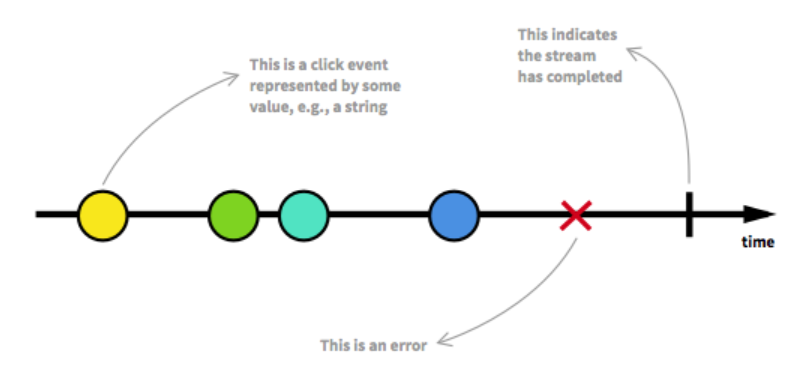
\includegraphics[width=12cm]{event-stream-diagram}
\caption{Ein Stream ist eine Sequenz von entstehenden Events geordnet nach der Zeit.}
\end{figure}

\noindent
Dabei kann ein Stream in Rx drei verschiedene Events ausstoßen:

\begin{itemize}
\item Wenn ein Wert ausgegeben wird,
\item Wenn ein Fehler ausgegeben wird,
\item wenn sich der Stream schließt.
\end{itemize}

\noindent
Diese Events können nur asynchron mit Hilfe von Funktionen festgehalten werden. Wenn man sich an einem Datenfluss anschließt, wird dies dann \textbf{subscribing} genannt. Der Stream ist dann entweder ein Observable oder ein Subject. 

\subsection{Observables}
Das Oben angeführte Beispiel wird nun in Code umgesetzt. Vor dem Ausführen des Beispiels muss folgend konfiguriert werden:

 \begin{center}
     Promises-vs.-Observables$\,\to\,$ webpack.config.js
 \end{center}
 
 \begin{figure}[H]
\begin{lstlisting}
module.exports = {
    mode: 'development',
    entry: './src/modules/observables/introduction.ts',
    ...
}
\end{lstlisting}
\end{figure}

 \begin{figure}[H]
\begin{lstlisting}
document.body.innerHTML += `<div class="center">
                                <input class="form-control" type="text">
                                <p id="result"></p>
                            </div>`;

const node = document.querySelector('input[type=text]');
const input$ = fromEvent(node, 'input');

input$.subscribe({
    next: event =>
        document.getElementById('result').innerText = (<HTMLInputElement> event.target).value,
    error: err => console.log(`Oops... ${err}`),
    complete: () => console.log(`Complete!`),
});
\end{lstlisting}
\end{figure}

\noindent
Das Observable-Objekt repräsentiert eine Kollektion die Werte zu seinen Beobachtern offenbart. In diesem Beispiel wird ein Input-Feld in die DOM eingefügt. Jedes mal wenn ein Wert in das Feld hinzugefügt wird, reagiert das Observable mit Hilfe des fromEvent-Operators darauf. In Echtzeit wird der Wert des Input-Feldes darunter angebunden.

\subsubsection{Push-vs. Pull-Prinzip}
\subsubsection{Hot Observables vs. Cold Observables}
\subsubsection{Unicast vs. Multicast}
\subsection{Operatoren}
\subsection{Subjects}









